\documentclass[11pt,a4paper]{article}
\usepackage[T1]{fontenc}
\usepackage[margin=2.2cm]{geometry}
\usepackage{graphicx,booktabs,float,array,enumitem,caption,fancyhdr,amsmath,tikz}
\usepackage[hidelinks]{hyperref}
\usetikzlibrary{positioning,arrows.meta,shapes.geometric}
\captionsetup{font=small,labelfont=bf}
\setlength{\parindent}{0pt}\setlength{\parskip}{5pt}
\pagestyle{fancy}\fancyhf{}
\lhead{Soft Computing MMCE30C3}
\cfoot{B.M.S.C.E Department of Computer Applications $|$ Page \thepage}
\renewcommand{\headrulewidth}{0.4pt}
\newcommand{\bx}[1]{\begin{tikzpicture}[baseline]\end{tikzpicture}}
\begin{document}
% ---------------- COVER ----------------
\thispagestyle{empty}
\begin{tikzpicture}[remember picture,overlay]
 \draw[line width=1.2pt] ([shift={(1.4,1.4)}]current page.south west) rectangle ([shift={(-1.4,-1.4)}]current page.north east);
 \draw[line width=0.5pt] ([shift={(1.55,1.55)}]current page.south west) rectangle ([shift={(-1.55,-1.55)}]current page.north east);
\end{tikzpicture}
\begin{center}
\vspace*{2.2cm}

\includegraphics[width=3.2cm]{logo.png}\\[0.8cm]
{\large\bfseries B. M. S. College of Engineering, Bengaluru-19}\\[3pt]
{\small (Autonomous College under VTU)}\\[2pt]
{\small Bull Temple Rd, Basavanagudi, Bengaluru, Karnataka 560019}\\[0.8cm]
{\bfseries Department of Computer Applications}\\[3pt]
{\bfseries 2025-2026}\\[0.9cm]
{\small Report is submitted for fulfilment of the Alternative Assessment Task (AAT) in the subject}\\[0.7cm]
{\Large\bfseries SOFT COMPUTING}\\[3pt]
{\large\bfseries (MMCE30C3)}\\[0.8cm]
{\small BY}\\[0.4cm]
\begin{tabular}{cc}
\textbf{Lohith S} & \textbf{Manjunath H}\\
{\small (1BM25MC052)} & {\small (1BM25MC054)}
\end{tabular}\\[0.8cm]
{\small Under the guidance of}\\[0.3cm]
{\bfseries Dr. K Vijayakumar}\\
{\small (Professor)}
\end{center}
\newpage
\tableofcontents
\newpage
% ---------------- TITLE ----------------
\begin{center}
{\Large\bfseries Early Sepsis Prediction in ICU Patients using a Hybrid of Genetic Algorithm, ANFIS and Particle Swarm Optimization}\\[4pt]
{\large Application of Soft Computing Techniques (AAT)}
\end{center}
\begin{center}
\begin{tabular}{|p{3.2cm}|p{10.5cm}|}
\hline
\textbf{Topic Name} & Early Sepsis Prediction using GA, ANFIS and PSO\\\hline
\textbf{Course} & MMCE30C3 -- Soft Computing\\\hline
\textbf{Semester} & III Semester MCA (Odd Semester 2026)\\\hline
\textbf{Student 1} & Lohith S (1BM25MC052)\\\hline
\textbf{Student 2} & Manjunath H (1BM25MC054)\\\hline
\textbf{Faculty} & Dr. K Vijayakumar, Professor\\\hline
\textbf{Tool Used} & Python on Google Colab (NumPy, Pandas, scikit-learn)\\\hline
\end{tabular}
\end{center}

\section{Introduction}
Sepsis is a serious condition in which the body reacts too strongly to an infection and starts damaging its own organs. It is one of the main causes of death in Intensive Care Units (ICUs). Every hour of delay in starting treatment reduces the chance of survival by about 7.6\%, so predicting sepsis a few hours early can save lives.

Building such a predictor is not easy for three reasons:
\begin{itemize}[nosep]
\item Sepsis is rare. Only about 2\% of the hourly ICU records are sepsis cases.
\item ICU data is noisy and has many missing values.
\item Doctors do not trust a model that gives a score without any reason.
\end{itemize}
In this project we solve the problem with soft computing. A fuzzy model (ANFIS) works with rules that a doctor can read. A Genetic Algorithm (GA) chooses which patient measurements to use, and Particle Swarm Optimization (PSO) tunes the fuzzy model. The model is trained on 20,336 ICU patients and tested on patients it has never seen, at the real sepsis rate.

\section{Objectives}
\begin{enumerate}[nosep]
\item To pick the most useful patient measurements, including 6-hour trends, using a Genetic Algorithm (GA).
\item To build a fuzzy rule based model (ANFIS) that gives a sepsis risk.
\item To train the fuzzy curves of that model using Particle Swarm Optimization (PSO).
\item To measure the result on unseen patients using AUROC, sensitivity, specificity, precision and time.
\item To compare the model with Logistic Regression and Random Forest on the same data.
\item To show, for a patient, which fuzzy rules caused the alert.
\end{enumerate}

\section{Soft Computing Models Used}
The project uses three techniques, one after the other. Figure~\ref{fig:flow} shows the overall flow.

\begin{figure}[H]
\centering
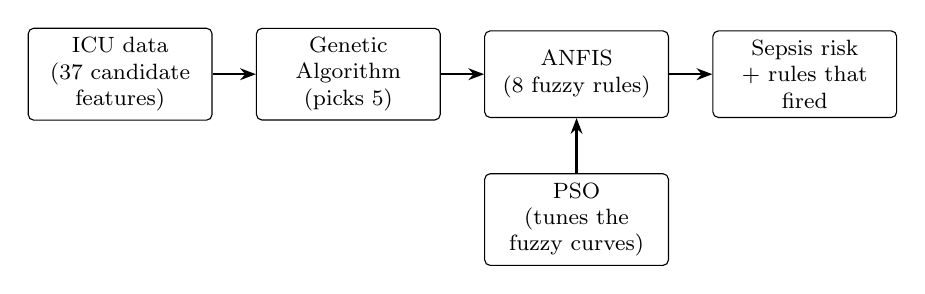
\begin{tikzpicture}[node distance=0.55cm,
 b/.style={draw,rounded corners=2pt,minimum height=1.1cm,text width=2.1cm,align=center,font=\footnotesize},
 a/.style={-{Stealth[length=2mm]},thick}]
 \node[b] (d) {ICU data\\(37 candidate features)};
 \node[b,right=of d] (g) {Genetic\\Algorithm\\(picks 5)};
 \node[b,right=of g] (n) {ANFIS\\(8 fuzzy rules)};
 \node[b,right=of n] (r) {Sepsis risk\\+ rules that\\fired};
 \node[b,below=0.7cm of n] (p) {PSO\\(tunes the\\fuzzy curves)};
 \draw[a] (d)--(g); \draw[a] (g)--(n); \draw[a] (n)--(r); \draw[a] (p)--(n);
\end{tikzpicture}
\caption{Overall flow of the model}\label{fig:flow}
\end{figure}

\subsection{Genetic Algorithm (GA): choosing the features}
We start with 37 candidate features: vital signs, lab values, how many times each lab was measured, and 6-hour trends of the vital signs. Using all of them would make the fuzzy model too big, so the GA picks between 3 and 6.
\begin{itemize}[nosep]
\item Each possible choice is a string of 37 bits: 1 means the feature is used, 0 means it is not.
\item A choice is scored by the AUROC of a quick logistic regression that uses only the chosen features, measured on separate patients, minus a small penalty for every extra feature.
\item Good choices are kept (tournament selection), mixed (uniform crossover) and slightly changed (mutation). This is repeated for 25 generations with a population of 30.
\end{itemize}

\subsection{ANFIS: the fuzzy rule model}
Instead of fixed limits like ``heart rate above 90 is high'', fuzzy logic says how much a value is high, from 0 to 1. ANFIS is a fuzzy system arranged like a small neural network. Our model has 8 rules of the form:

\emph{IF HR is like $A_r$ AND BUN is like $B_r$ AND \dots{} THEN risk is $f_r$ (a small linear formula).}

\begin{enumerate}[nosep]
\item \textbf{Rules from k-means:} patients are grouped into 8 natural groups, and each group becomes one rule.
\item \textbf{Fuzzify:} each input is converted to a degree between 0 and 1 using a bell shaped (Gaussian) curve with a centre $c$ and a width $\sigma$.
\item \textbf{Rule strength:} the degrees of one rule are multiplied, and the strengths of all rules are scaled to add up to 1.
\item \textbf{Combine:} the output of each rule is added, with the stronger rules counting more. The linear formulas of the rules are found by least squares (Jang's hybrid learning).
\item \textbf{Risk:} the final score is changed into a probability using Platt scaling (a sigmoid fitted on validation patients).
\end{enumerate}

\subsection{Particle Swarm Optimization (PSO): tuning the model}
The model has 80 curve numbers (8 rules $\times$ 5 inputs $\times$ centre and width) that must be set correctly. Normal gradient training does not work well for this, so we use PSO.
\begin{itemize}[nosep]
\item 40 particles are created. Each particle is one full set of curve numbers. One particle starts from the k-means solution, some start near it, the rest start random.
\item Every particle moves a little in each round. It is pulled towards the best set it has found itself and towards the best set found by the whole swarm. The inertia is reduced from 0.9 to 0.4, so the swarm explores first and settles later.
\item Particles are judged by $(1-\text{AUROC}) + 0.1\times$ weighted squared error on separate patients. Sepsis cases are given more weight because they are rare.
\item This is repeated for 60 rounds and the best set is kept.
\end{itemize}

\begin{figure}[H]
\centering
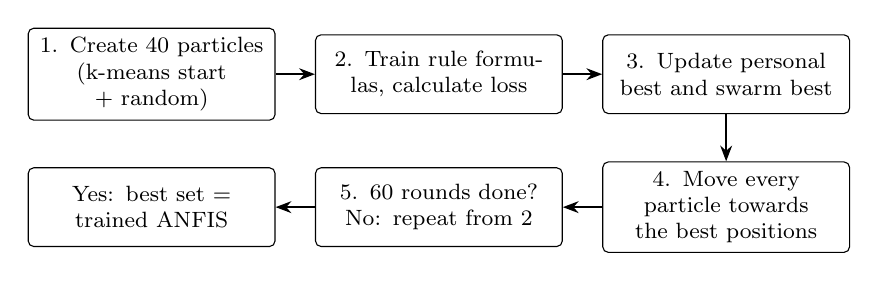
\begin{tikzpicture}[node distance=0.5cm,
 b/.style={draw,rounded corners=2pt,minimum height=1cm,text width=2.9cm,align=center,font=\footnotesize},
 a/.style={-{Stealth[length=2mm]},thick}]
 \node[b] (1) {1. Create 40 particles\\(k-means start + random)};
 \node[b,right=of 1] (2) {2. Train rule formulas, calculate loss};
 \node[b,right=of 2] (3) {3. Update personal best and swarm best};
 \node[b,below=0.6cm of 3] (4) {4. Move every particle towards the best positions};
 \node[b,left=of 4] (5) {5. 60 rounds done? No: repeat from 2};
 \node[b,left=of 5] (6) {Yes: best set = trained ANFIS};
 \draw[a] (1)--(2); \draw[a] (2)--(3); \draw[a] (3)--(4); \draw[a] (4)--(5); \draw[a] (5)--(6);
\end{tikzpicture}
\caption{Working of PSO}
\end{figure}

\section{Data Set Used}
We used the PhysioNet / Computing in Cardiology Challenge 2019 sepsis data set (Training Set A), taken from \url{https://physionet.org/content/challenge-2019/1.0.0/}. It has hourly ICU records with vital signs, lab values and a label \texttt{SepsisLabel} that is 1 from 6 hours before sepsis starts.

\begin{table}[H]
\centering\small
\caption{Data set details and preparation}
\begin{tabular}{@{}p{4.2cm}p{11cm}@{}}
\toprule
\textbf{Item} & \textbf{Detail}\\\midrule
Patients used & All 20,336 patient files (1,790 patients developed sepsis)\\
Hourly records & 790,215; sepsis records 17,136 (2.17\%)\\
Split & 60\% train, 20\% validation, 20\% test, \textbf{by patient} (no patient appears in two parts)\\
Validation / test rows & 157,812 / 159,397 at the natural sepsis rate (test: 2.14\%)\\
Training rows for GA and PSO & 12,000 rows to learn, 7,500 rows to judge candidates (all from training patients; sepsis rows over-sampled)\\
Candidate features & 37: HR, O2Sat, Temp, SBP, MAP, DBP, Resp, WBC, Lactate, Creatinine, Platelets, BUN, Shock Index, Age, ICU hours (ICULOS), lab measurement counts, 6-hour change, mean and variability of the vital signs\\
Missing values & Filled with the last known value of the patient, then the median of the training patients\\
Scaling & Standardised using training patients only (mean 0, standard deviation 1)\\\bottomrule
\end{tabular}
\end{table}

\section{Implementation}
The whole program was written in Python (NumPy, Pandas, scikit-learn) on Google Colab. The steps are:
\begin{enumerate}[nosep]
\item Download and load all 20,336 patient files (790,215 records).
\item Clean the data, add Shock Index, lab counts and 6-hour trends, then scale.
\item Split the patients into train, validation and test groups.
\item Genetic Algorithm selects 5 features: HR, BUN, ICULOS, Resp\_m6 (6-hour mean respiration rate) and Temp\_s6 (6-hour variability of temperature).
\item Build the ANFIS with 8 rules using k-means.
\item Tune the fuzzy curves with PSO (40 particles, 60 rounds).
\item Choose the alert threshold on the validation patients so that about 80\% of sepsis records are caught.
\item Test once on the unseen test patients and compare with Logistic Regression and Random Forest.
\item Check sample patients: risk and the rules that fired.
\end{enumerate}

\section{Results and Screenshots}
\subsection{GA and PSO output}
\begin{table}[H]
\centering\small
\caption{GA and PSO stages}
\begin{tabular}{@{}p{7.5cm}p{7.5cm}@{}}
\toprule
\textbf{Item} & \textbf{Value}\\\midrule
Features selected by GA (from 37) & HR, BUN, ICULOS, Resp\_m6, Temp\_s6\\
GA time & 14.6 s\\
Quick logistic regression AUROC (5 GA features / all 37) & 0.7213 / 0.7287\\
PSO loss, k-means start $\rightarrow$ after 60 rounds & 0.2848 $\rightarrow$ 0.2435\\
Validation AUROC, k-means rules only $\rightarrow$ after PSO & 0.7164 $\rightarrow$ 0.7283\\
PSO training time & 98.1 s\\\bottomrule
\end{tabular}
\end{table}
The GA reduced 37 features to 5, and these 5 give almost the same AUROC as all 37 (0.7213 against 0.7287). PSO lowered the training loss in every stage and improved the validation AUROC over the k-means rules alone.

\begin{figure}[H]
\centering
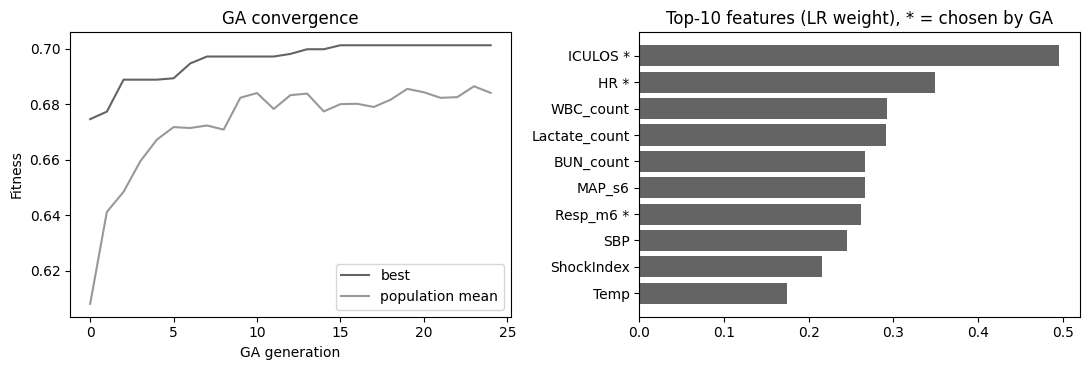
\includegraphics[width=\textwidth]{fig2.png}
\caption{GA convergence (left) and the 10 features with the largest logistic regression weights; * marks the features chosen by the GA (right)}
\end{figure}

\subsection{Test results (159,397 unseen records)}
The alert threshold was chosen on validation patients as a risk of 1.33\%, which catches about 80\% of sepsis records. The same rule was used for every model.

\begin{table}[H]
\centering\small
\caption{Performance on the test patients (natural sepsis rate 2.14\%)}
\begin{tabular}{@{}lccccccc@{}}
\toprule
\textbf{Model} & \textbf{AUROC} & \textbf{AUPRC} & \textbf{Sens.\%} & \textbf{Spec.\%} & \textbf{Prec.\%} & \textbf{Acc.\%} & \textbf{FA/TA}\\\midrule
\textbf{GA+ANFIS+PSO (ours)} & \textbf{0.7547} & \textbf{0.0860} & 83.7 & 45.8 & 3.3 & 46.6 & 29.6\\
Logistic Regression (GA features) & 0.7270 & 0.0835 & 84.3 & 37.4 & 2.9 & 38.4 & 33.9\\
Random Forest (GA features) & 0.7642 & 0.0994 & 85.0 & 45.6 & 3.3 & 46.5 & 29.2\\
Logistic Regression (all features) & 0.7483 & 0.0929 & 82.6 & 45.3 & 3.2 & 46.1 & 30.3\\
Random Forest (all features) & 0.8100 & 0.1107 & 82.5 & 61.3 & 4.5 & 61.8 & 21.4\\\bottomrule
\end{tabular}

\smallskip
{\footnotesize Sens. = sensitivity, Spec. = specificity, Prec. = precision, Acc. = accuracy, FA/TA = false alarms per true alert. AUPRC of a random model is 0.021.}
\end{table}

\begin{table}[H]
\centering\small
\caption{Confusion matrix of the ANFIS model on the test data}
\begin{tabular}{@{}lcc@{}}
\toprule
 & \textbf{Predicted: No sepsis} & \textbf{Predicted: Sepsis}\\\midrule
\textbf{Actual: No sepsis} & 71,461 (TN) & 84,522 (FP)\\
\textbf{Actual: Sepsis} & 556 (FN) & 2,858 (TP)\\\bottomrule
\end{tabular}
\end{table}

Prediction of one record takes 1.48 $\mu$s, and the full training (GA + PSO) takes about 113 s.

\begin{figure}[H]
\centering
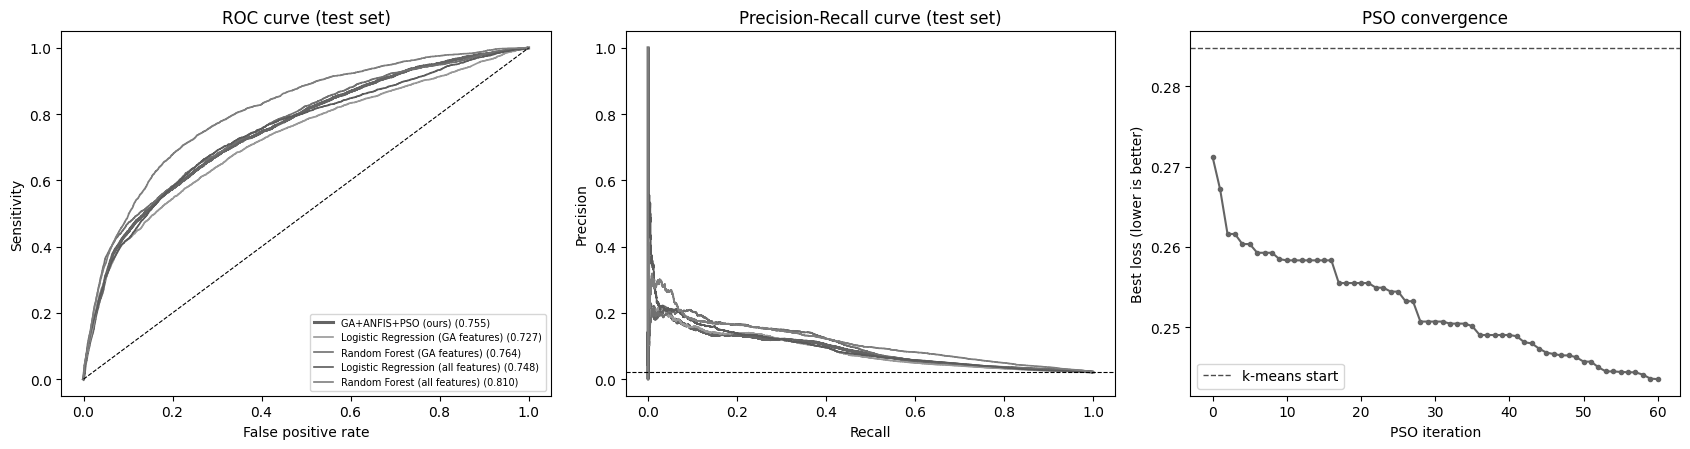
\includegraphics[width=\textwidth]{fig1.png}
\caption{ROC curve (left), precision-recall curve (middle) and PSO convergence (right) on the test patients. The thick line is the proposed model.}
\end{figure}

\subsection{Rules learned by the model}
After training, each of the 8 rules is a patient profile. Table~\ref{tab:rules} shows the centre of the fuzzy curve of each input in real units.

\begin{table}[H]
\centering\small
\caption{Fuzzy rule centres after PSO (real units)}\label{tab:rules}
\begin{tabular}{@{}lccccc@{}}
\toprule
\textbf{Rule} & \textbf{HR} & \textbf{BUN} & \textbf{ICULOS (h)} & \textbf{Resp\_m6} & \textbf{Temp\_s6}\\\midrule
1 & 87.7 & 3.6 & 38.8 & 21.3 & 0.3\\
2 & 75.3 & 15.3 & 1.0 & 18.9 & 0.8\\
3 & 101.0 & 9.4 & 50.8 & 15.8 & 0.2\\
4 & 48.5 & 1.0 & 104.1 & 17.4 & 0.0\\
5 & 84.4 & 76.7 & 34.0 & 20.2 & 0.0\\
6 & 87.4 & 34.6 & 118.2 & 21.9 & 0.2\\
7 & 94.0 & 25.8 & 13.0 & 18.2 & 0.4\\
8 & 102.0 & 2.6 & 12.4 & 26.2 & 0.3\\\bottomrule
\end{tabular}
\end{table}

For example, Rule 8 reads: \emph{IF heart rate is high (about 102) AND ICU stay is short (about 12 hours) AND recent respiration rate is high (about 26) THEN add its risk formula.}

\subsection{Testing with sample patients}
Two real patients from the test group were given to the trained model. An alert is raised when the risk is 1.33\% or more.

\begin{table}[H]
\centering\small
\caption{Sample patient predictions}
\begin{tabular}{@{}lcc@{}}
\toprule
 & \textbf{Patient A (developing sepsis)} & \textbf{Patient B (stable)}\\\midrule
HR / BUN / ICULOS & 87 / 14 / 117 & 72 / 17 / 3\\
Resp\_m6 / Temp\_s6 & 17.0 / 0.0 & 16.5 / 0.0\\
Sepsis risk & 7.50\% & 0.90\%\\
Decision & Alert & Normal\\
Main rule & Rule 6 (100\%) & Rule 2 (46.6\%), Rule 6 (about 44\%)\\\bottomrule
\end{tabular}
\end{table}

\begin{figure}[H]
\centering
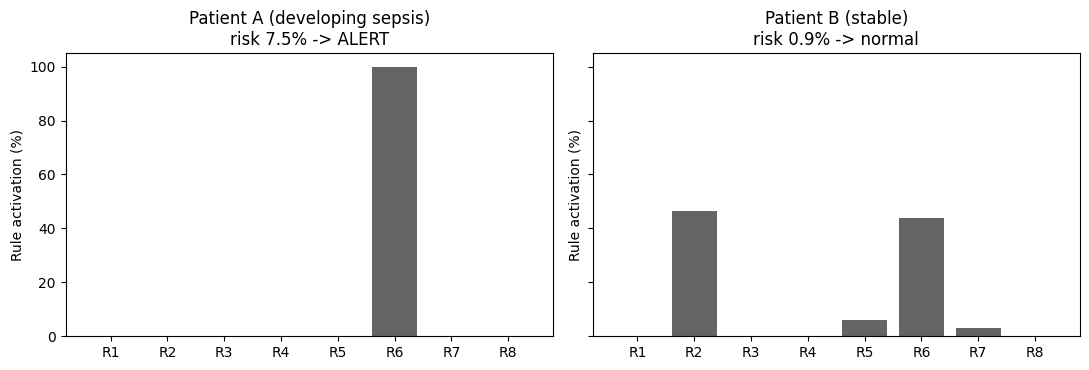
\includegraphics[width=0.95\textwidth]{fig3.png}
\caption{Fuzzy rule activation for the two sample patients}
\end{figure}

\section{Interpretation and Conclusions}
\begin{itemize}[nosep]
\item The model reached an AUROC of 0.7547 on 159,397 unseen records at the real 2\% sepsis rate, against 0.61 for our first version that used 3 inputs and 2,000 patients. It also caught 83.7\% of sepsis records.
\item The model is better than Logistic Regression on all 37 features (0.7483) and on the same 5 features (0.7270). Random Forest on the same 5 features reached 0.7642, so the fuzzy model is close to it while giving readable rules. Random Forest on all features is the best model (0.8100), but it cannot explain an alert with rules.
\item The GA found that 5 of 37 features are enough. PSO improved the model over the k-means rules alone (validation AUROC 0.7164 to 0.7283), and the PSO loss was still falling after 60 rounds.
\item Accuracy (46.6\%) looks low because the threshold was chosen to catch most sepsis cases. A model that always says ``no sepsis'' would have 98\% accuracy and would be useless, so AUROC, sensitivity and precision-recall are the right measures here.
\item The precision is low (3.3\%): there are about 30 false alarms for every true alert, and when alerts are checked every hour almost all patients get at least one alert. The model is therefore a risk ranking tool for support, not a diagnosis.
\item The GA selected ICULOS (hours in the ICU). This is a time indicator, not a body measurement: sepsis becomes more likely the longer a patient stays. The sample patient A was alerted mainly because of a long ICU stay and BUN, not because of abnormal vital signs.
\item The rules explain every alert, training takes about 2 minutes and one prediction takes about 1.5 $\mu$s, so the model can run in real time.
\item \textbf{Limitations:} only Training Set A was used and the result is from one run; the validation AUROC (0.728) and test AUROC (0.755) differ because they are different groups of patients; alerts are made hour by hour without a rule for repeated alerts. Future work: alert only after several high-risk hours, more PSO rounds and rules, and Training Set B.
\end{itemize}

\section{Colab Notebook (Trained Model)}
The complete code, the trained model and all the outputs shown in this report are available in the Google Colab notebook below. This notebook is where the model was trained and tested.

\url{https://colab.research.google.com/drive/129Vp54XgDU9ZiHHvMUUENfBy1j8-nXZj?usp=sharing}

\begin{thebibliography}{9}
\bibitem{r1} M. Reyna et al., ``Early Prediction of Sepsis from Clinical Data: The PhysioNet/Computing in Cardiology Challenge 2019,'' \emph{Critical Care Medicine}, vol. 48, no. 2, pp. 210--217, 2020.
\bibitem{r2} J.-S. R. Jang, ``ANFIS: Adaptive-Network-Based Fuzzy Inference System,'' \emph{IEEE Transactions on Systems, Man, and Cybernetics}, vol. 23, no. 3, pp. 665--685, 1993.
\bibitem{r3} J. Kennedy and R. Eberhart, ``Particle Swarm Optimization,'' in \emph{Proc. IEEE International Conference on Neural Networks}, 1995, pp. 1942--1948.
\bibitem{r4} D. E. Goldberg, \emph{Genetic Algorithms in Search, Optimization, and Machine Learning}, Addison-Wesley, 1989.
\bibitem{r5} L. Breiman, ``Random Forests,'' \emph{Machine Learning}, vol. 45, no. 1, pp. 5--32, 2001.
\bibitem{r6} Department of Computer Applications, Guidelines for AAT: Soft Computing (MMCE30C3), B.M.S. College of Engineering, Bengaluru, 2026.
\end{thebibliography}
\end{document}
